% SC4022 --- Chapter 3: Community Detection (0->100 ground-up)
\chapter{Community Detection}
\label{ch:community}
\sloppy

\begin{quote}
\emph{``Birds of a feather flock together.''} --- Social circles, protein complexes, and Web topics all appear as clusters: many links inside, few between. Finding those clusters automatically is community detection.
\end{quote}

\noindent\fbox{\parbox{\dimexpr\linewidth-2\fboxsep-2\fboxrule}{%
\textbf{From zero: we build here, no clustering background needed.} We assume only Ch.~1--2 (graph, degree, paths). Every notion---community, modularity, spectral cut---is introduced by picture, then defined, then exercised.}}
\vspace{0.4em}

\section*{Learning Outcomes}
After this chapter you will be able to:
\begin{enumerate}[label=(L\arabic*)]
    \item define community structure and explain why ``dense inside, sparse outside'' matters;
    \item formulate modularity $Q$ and compute it on small partitions by hand;
    \item run one step of Louvain greedy optimisation and trace label propagation;
    \item apply spectral bisection via the graph Laplacian and Fiedler vector;
    \item evaluate partitions with NMI, adjusted Rand, and conductance.
\end{enumerate}

% ============================================================
\section{What Is a Community?}
\label{sec:what-community}
\paragraph{Intuition.} Look at Fig.~\ref{fig:two-comms}: two triangles linked by a single edge. Inside each triangle every pair is connected (dense); between triangles there is one bridge (sparse). If you delete that bridge, the network splits cleanly. A \emph{community} is such a piece---more edges than you would expect by chance. The challenge: formalise ``than expected'' so a computer can search for it.

We need a \emph{null model}: what would the edge pattern look like if there were no communities but degrees were preserved? The \emph{configuration model} (Ch.~4) randomises edges while keeping each node's degree, so an edge between high-degree nodes is less surprising than one between low-degree nodes. Modularity counts surprise.

\begin{definition}[Modularity $Q$]\label{def:modularity}
For partition $\mathcal{C}=\{c_i\}$ where $c_i$ is the community of node $i$, with adjacency $A_{ij}$ and $m=|E|$,
\begin{equation}
Q=\frac1{2m}\sum_{ij}\Bigl[A_{ij}-\frac{k_i k_j}{2m}\Bigr]\,\delta(c_i,c_j),
\end{equation}
where $\delta(c_i,c_j)=1$ if $c_i=c_j$, else $0$. Equivalently $Q=\sum_{c}(e_{cc}-a_c^2)$ with $e_{cc}$ = fraction of edges inside $c$ and $a_c$ = fraction of edge-ends in $c$. Range $Q\in[-1/2,1]$; $Q>0.3$ often indicates meaningful communities; $Q\approx0$ suggests none.
\end{definition}

\begin{figure}[h]\centering
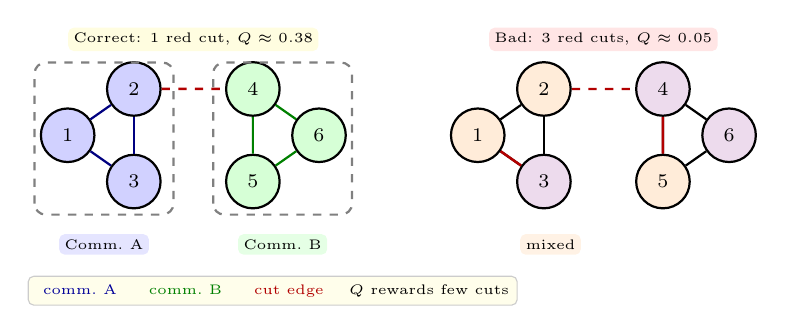
\begin{tikzpicture}[scale=0.84,every node/.style={font=\scriptsize}]
% left community - correct partition
\begin{scope}
\node[circle,draw,thick,fill=blue!18,minimum size=0.68cm] (a1) at (0,1.2) {1};
\node[circle,draw,thick,fill=blue!18,minimum size=0.68cm] (a2) at (1.0,1.9) {2};
\node[circle,draw,thick,fill=blue!18,minimum size=0.68cm] (a3) at (1.0,0.5) {3};
\node[circle,draw,thick,fill=green!16,minimum size=0.68cm] (b1) at (2.8,1.9) {4};
\node[circle,draw,thick,fill=green!16,minimum size=0.68cm] (b2) at (2.8,0.5) {5};
\node[circle,draw,thick,fill=green!16,minimum size=0.68cm] (b3) at (3.8,1.2) {6};
\draw[thick,blue!50!black] (a1)--(a2); \draw[thick,blue!50!black] (a2)--(a3); \draw[thick,blue!50!black] (a1)--(a3);
\draw[thick,green!50!black] (b1)--(b2); \draw[thick,green!50!black] (b1)--(b3); \draw[thick,green!50!black] (b2)--(b3);
\draw[thick,red!70!black,dashed,line width=0.9pt] (a2)--(b1);
\draw[dashed,gray,thick,rounded corners=4pt] (-0.5,0.0) rectangle (1.6,2.3);
\draw[dashed,gray,thick,rounded corners=4pt] (2.2,0.0) rectangle (4.3,2.3);
\node[font=\tiny,fill=blue!10,rounded corners=2pt,inner sep=2pt] at (0.55,-0.45) {Comm.~A};
\node[font=\tiny,fill=green!10,rounded corners=2pt,inner sep=2pt] at (3.25,-0.45) {Comm.~B};
\node[font=\tiny,fill=yellow!12,rounded corners=2pt,inner sep=2pt] at (1.9,2.65) {Correct: 1 red cut, $Q\approx0.38$};
\end{scope}
% right - bad partition
\begin{scope}[xshift=6.2cm]
\node[circle,draw,thick,fill=orange!15,minimum size=0.68cm] (c1) at (0,1.2) {1};
\node[circle,draw,thick,fill=orange!15,minimum size=0.68cm] (c2) at (1.0,1.9) {2};
\node[circle,draw,thick,fill=violet!14,minimum size=0.68cm] (c3) at (1.0,0.5) {3};
\node[circle,draw,thick,fill=violet!14,minimum size=0.68cm] (d1) at (2.8,1.9) {4};
\node[circle,draw,thick,fill=orange!15,minimum size=0.68cm] (d2) at (2.8,0.5) {5};
\node[circle,draw,thick,fill=violet!14,minimum size=0.68cm] (d3) at (3.8,1.2) {6};
\draw[thick] (c1)--(c2); \draw[thick] (c2)--(c3); \draw[thick] (c1)--(c3);
\draw[thick] (d1)--(d2); \draw[thick] (d1)--(d3); \draw[thick] (d2)--(d3);
\draw[thick,red!70!black,dashed] (c2)--(d1);
\draw[thick,red!70!black,line width=0.9pt] (c1)--(c3); \draw[thick,red!70!black,line width=0.9pt] (d1)--(d2);
\node[font=\tiny,fill=red!10,rounded corners=2pt,inner sep=2pt] at (1.9,2.65) {Bad: 3 red cuts, $Q\approx0.05$};
\node[font=\tiny,fill=orange!10,rounded corners=2pt,inner sep=2pt] at (1.1,-0.45) {mixed};
\end{scope}
\node[font=\tiny,draw=gray!40,fill=yellow!8,rounded corners=2pt,inner sep=3pt] at (3.1,-1.15) {\textcolor{blue!60!black}{$\blacksquare$ comm.~A} \quad \textcolor{green!50!black}{$\blacksquare$ comm.~B} \quad \textcolor{red!70!black}{$\blacksquare$ cut edge} \quad $Q$ rewards few cuts};
\end{tikzpicture}
\caption{Two partitions of the same 6-node graph. Left: each triangle is a community---one cut edge, high modularity. Right: mixing nodes across triangles---three cuts, low $Q$. Modularity formalises ``surprisingly dense inside.''}
\label{fig:two-comms}
\end{figure}

\begin{example}[Modularity by hand]\label{ex:mod-by-hand}
Take left partition in Fig.~\ref{fig:two-comms}: $m=7$ edges, $k_i=2$ for leaves and $3$ for the two bridge nodes (2 and 4). For community $A=\{1,2,3\}$, $e_{AA}=3/7$, $a_A=(2+3+2)/(2\cdot7)=7/14=0.5$; similarly $a_B=0.5$, $e_{BB}=3/7$. So $Q=(3/7-0.25)+(3/7-0.25)\approx0.36$. Right partition splits triangles, giving $Q\approx0.05$---much worse, as expected.
\end{example}

% ============================================================
\section{Louvain and Label Propagation}
\label{sec:louvain}
\paragraph{Intuition for Louvain.} Start with each node alone. Repeatedly try moving a node to a neighbour's community if $Q$ increases; when no move helps, collapse each community into a super-node and repeat. This greedy hill-climbing is fast ($O(m)$ per pass) and finds high-$Q$ partitions on large graphs. The Leiden variant adds a refinement step to guarantee connected communities.

\paragraph{Intuition for label propagation.} Give each node a unique label, then repeatedly let each node adopt the most frequent label among neighbours (ties broken randomly). Dense regions quickly agree on one label; boundaries oscillate. It is near-linear and needs no parameter, but results vary with update order.

\begin{figure}[h]\centering
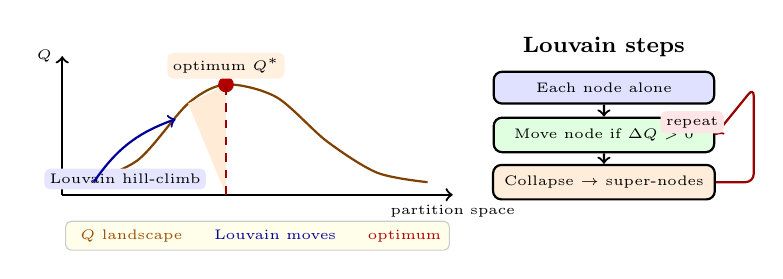
\begin{tikzpicture}[scale=0.80,every node/.style={font=\scriptsize}]
% modularity landscape
\draw[->,thick] (0,0)--(6.2,0) node[below,font=\tiny] {partition space};
\draw[->,thick] (0,0)--(0,2.2) node[left,font=\tiny] {$Q$};
\draw[thick,orange!50!black,smooth] plot coordinates {(0.3,0.15) (1.2,0.55) (2.0,1.45) (2.6,1.75) (3.4,1.55) (4.2,0.85) (5.0,0.35) (5.8,0.20)};
\fill[orange!16] (2.6,0)--(2.6,1.75)--(2.0,1.45)--cycle;
\node[circle,fill=red!70!black,inner sep=2pt] at (2.6,1.75) {};
\node[font=\tiny,fill=orange!12,rounded corners=2pt,inner sep=2pt] at (2.6,2.05) {optimum $Q^*$};
\draw[dashed,red!60!black] (2.6,0)--(2.6,1.75);
\node[font=\tiny,fill=blue!10,rounded corners=2pt,inner sep=2pt] at (1.0,0.25) {Louvain hill-climb};
\draw[->,thick,blue!60!black] (0.5,0.20) to[bend left=18] (1.8,1.20);
% side: Louvain steps
\begin{scope}[xshift=7.2cm]
\node[font=\footnotesize\bfseries] at (1.4,2.35) {Louvain steps};
\node[draw,thick,fill=blue!12,rounded corners=3pt,minimum width=2.8cm,align=center,inner sep=4pt,font=\tiny] (s1) at (1.4,1.7) {Each node alone};
\node[draw,thick,fill=green!12,rounded corners=3pt,minimum width=2.8cm,align=center,inner sep=4pt,font=\tiny] (s2) at (1.4,0.95) {Move node if $\Delta Q>0$};
\node[draw,thick,fill=orange!14,rounded corners=3pt,minimum width=2.8cm,align=center,inner sep=4pt,font=\tiny] (s3) at (1.4,0.20) {Collapse $\to$ super-nodes};
\draw[->,thick] (s1)--(s2); \draw[->,thick] (s2)--(s3);
\draw[->,thick,red!60!black,rounded corners=3pt] (s3.east) -- ++(0.6,0) -- ++(0,1.5) -- (s2.east);
\node[font=\tiny,fill=red!10,rounded corners=2pt,inner sep=2pt] at (2.8,1.15) {repeat};
\end{scope}
\node[font=\tiny,draw=gray!40,fill=yellow!8,rounded corners=2pt,inner sep=3pt] at (3.1,-0.65) {\textcolor{orange!60!black}{$\blacksquare$ $Q$ landscape} \quad \textcolor{blue!60!black}{$\blacksquare$ Louvain moves} \quad \textcolor{red!70!black}{$\blacksquare$ optimum}};
\end{tikzpicture}
\caption{Modularity optimisation as hill-climbing. Left: $Q$ rises to an optimum then falls as partitions over-merge. Louvain moves single nodes greedily, collapses communities, and repeats. Leiden adds refinement to avoid disconnected communities.}
\label{fig:mod-landscape}
\end{figure}

% ============================================================
\section{Spectral Partitioning}
\label{sec:spectral}
\paragraph{Intuition.} Place nodes on a line so connected nodes stay close; then cut the line in the middle. The Laplacian $L=D-A$ (degree matrix minus adjacency) measures ``stretch''; its second-smallest eigenvector (Fiedler vector) gives the best 1-D placement.

\begin{definition}[Graph Laplacian and Fiedler cut]\label{def:laplacian}
Let $D=\mathrm{diag}(k_1,\dots,k_n)$. The \emph{Laplacian} is $L=D-A$, symmetric positive semidefinite, with eigenvalues $0=\lambda_1\le\lambda_2\le\cdots\le\lambda_n$. The \emph{Fiedler vector} $f$ satisfies $Lf=\lambda_2 f$, $\sum_i f_i=0$. Spectral bisection puts $i$ in $S$ if $f_i\ge0$, else $\bar S$. Small $\lambda_2$ signals a good cut (nearly disconnected); large $\lambda_2$ means well-connected (expander).
\end{definition}

\begin{figure}[h]\centering
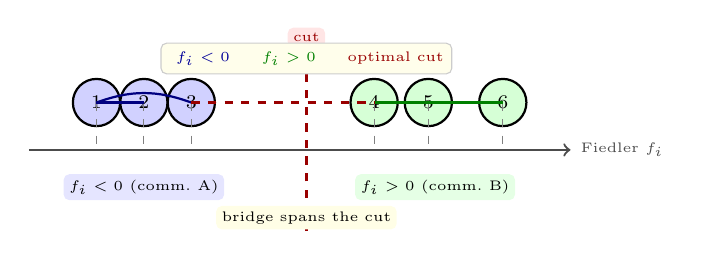
\begin{tikzpicture}[scale=0.86,every node/.style={font=\scriptsize}]
% spectral line
\draw[thick,->,gray!60!black] (-0.5,0)--(7.5,0) node[right,font=\tiny] {Fiedler $f_i$};
\draw[thick,dashed,red!60!black] (3.6,-1.2)--(3.6,1.5) node[above,font=\tiny,fill=red!10,rounded corners=2pt,inner sep=2pt] {cut};
% left community nodes
\foreach \x/\n in {0.5/1,1.2/2,1.9/3} {\node[circle,draw,thick,fill=blue!18,minimum size=0.6cm] at (\x,0.7) {\n}; \draw[thin,gray,dashed] (\x,0.7)--(\x,0);}
\foreach \x/\n in {4.6/4,5.4/5,6.5/6} {\node[circle,draw,thick,fill=green!16,minimum size=0.6cm] at (\x,0.7) {\n}; \draw[thin,gray,dashed] (\x,0.7)--(\x,0);}
% edges among left and right + bridge
\draw[thick,blue!50!black] (0.5,0.7) to[bend left=20] (1.9,0.7); \draw[thick,blue!50!black] (0.5,0.7)--(1.2,0.7);
\draw[thick,green!50!black] (4.6,0.7)--(5.4,0.7); \draw[thick,green!50!black] (5.4,0.7)--(6.5,0.7);
\draw[thick,red!60!black,dashed] (1.9,0.7)--(4.6,0.7);
\node[font=\tiny,fill=blue!10,rounded corners=2pt,inner sep=2pt] at (1.2,-0.55) {$f_i<0$ (comm.~A)};
\node[font=\tiny,fill=green!10,rounded corners=2pt,inner sep=2pt] at (5.5,-0.55) {$f_i>0$ (comm.~B)};
\node[font=\tiny,fill=yellow!10,rounded corners=2pt,inner sep=2pt] at (3.6,-1.0) {bridge spans the cut};
\node[font=\tiny,draw=gray!40,fill=yellow!8,rounded corners=2pt,inner sep=3pt] at (3.6,1.35) {\textcolor{blue!60!black}{$\blacksquare$ $f_i<0$} \quad \textcolor{green!50!black}{$\blacksquare$ $f_i>0$} \quad \textcolor{red!60!black}{$\blacksquare$ optimal cut}};
\end{tikzpicture}
\caption{Spectral embedding: the Fiedler vector places nodes on a line; sign gives the bisection. Nodes 1--3 fall left of zero, 4--6 right; the bridge edge $3$--$4$ is the only one crossing, so conductance is minimal.}
\label{fig:spectral-line}
\end{figure}

% ============================================================
\section{Evaluating Partitions}
\label{sec:evaluating}
When ground-truth communities are known (e.g.\ planted partition or karate labels), compare with \emph{normalised mutual information} (NMI, 1 = identical) or \emph{adjusted Rand index} (ARI). Without ground truth, use \emph{conductance} $\phi(S)=|\text{cut}(S,\bar S)|/\min(\text{vol}(S),\text{vol}(\bar S))$ (small = good community) and coverage. Modularity itself is a score but should not be the sole evaluation---it has a resolution limit: it merges small communities in large graphs.

\begin{lstlisting}[language=Python, caption={Louvain communities and modularity on the karate club.}, label={lst:louvain}]
import networkx as nx
import community as community_louvain  # python-louvain

G = nx.karate_club_graph()
part = community_louvain.best_partition(G)  # dict node -> comm id
mod = community_louvain.modularity(part, G)
print(f"communities: {len(set(part.values()))}  Q={mod:.3f}")
# Show sizes
from collections import Counter
print(Counter(part.values()))
# Louvain step intuition: try moving node 0 and check delta Q
\end{lstlisting}

\begin{lstlisting}[language=Python, caption={Spectral bisection via the Laplacian Fiedler vector.}, label={lst:spectral}]
import networkx as nx
import numpy as np

G = nx.karate_club_graph()
L = nx.laplacian_matrix(G).toarray()
w, V = np.linalg.eigh(L)          # eigenvalues sorted
fiedler = V[:, 1]                  # second smallest
# Bisection by sign
comm = {i: int(fiedler[i] >= 0) for i in range(len(fiedler))}
# Conductance of this cut
S = {i for i,c in comm.items() if c==0}
cut = sum(1 for u,v in G.edges() if (u in S) != (v in S))
vol_S = sum(dict(G.degree(S)).values())
vol_rest = 2*G.number_of_edges() - vol_S
print(f"lambda2={w[1]:.3f} cut={cut} conductance={cut/min(vol_S,vol_rest):.3f}")
\end{lstlisting}

\begin{remark}[Overlapping communities]\label{rem:overlap}
A node may belong to several groups (family, lab, sports). Extensions like clique percolation or mixed-membership SBM allow $c_i$ to be a distribution over communities. Louvain and spectral cuts are disjoint; overlapping scores need generalised modularity or NMI variants.
\end{remark}

% ============================================================
\section{Chapter Notes}
Modularity was introduced by Newman \& Girvan (2004) and Newman (2006); Louvain by Blondel et~al.\ (2008) and Leiden by Traag et~al.\ (2019). Spectral partitioning originates with Fiedler (1973) and the Cheeger inequality linking $\lambda_2$ to conductance. The resolution limit (Fortunato \& Barth\'elemy, 2007) warns that $Q$ optimisation merges communities smaller than $\sqrt{2m}$. Overlapping methods (clique percolation, MMSB) address nodes belonging to many groups.

% ============================================================
\section{Exercises}
\label{sec:ch03-exercises}
\begin{enumerate}[label=E3.\arabic*, leftmargin=*, itemsep=0.8em]
    \item \textbf{Modularity by hand.} For Fig.~\ref{fig:two-comms} left (two triangles, one bridge, $m=7$), compute $Q$ for: (a) the correct two-community split, (b) all nodes in one community, (c) each node alone. Which is highest? Why does (b) give $Q=0$?
    \item \textbf{Louvain trace.} Start with 6 singleton communities on Fig.~\ref{fig:two-comms}. Consider moving node $2$ into community $\{1,3\}$: compute $\Delta Q$ (formula or brute force with code). Would Louvain accept this move on the first pass?
    \item \textbf{Fiedler sign.} Build the 6-node two-triangle graph in NetworkX, compute Laplacian eigenvalues, and verify $\lambda_2>0$ (connected). Report the Fiedler vector and check that its sign matches the natural bisection.
    \item \textbf{NMI vs modularity.} On the karate club, compare Louvain's partition to the ground-truth ``Mr.~Hi vs John A'' split (node attribute `club`). Compute NMI (sklearn) and modularity for both. Which score favours which partition and why?
    \item \textbf{Resolution limit.} Consider a ring of $k$ cliques each of size $c$, linked in a cycle by one edge between successive cliques. For large $k$, Newman shows Louvain merges adjacent cliques despite clear structure. Explain why $Q$ prefers merging when $c<\sqrt{2m}$ and test with $c=4$, $k=10$ in code.
\end{enumerate}
% End of Chapter 3
